% Scalar instruction entry source: tools/generate_scalar_instruction_catalog.py.
\subsection{\texttt{SB.PCR}}
\label{sec:scalar-sb_pcr}
\index{SB.PCR@\texttt{SB.PCR}}
\begin{sloppypar}\noindent\textbf{Purpose.} Stores a 8-bit value to memory using PC-relative/symbol addressing.\end{sloppypar}\smallskip
\noindent\textbf{Syntax.}\par
\begin{lstlisting}[style=ptoscalarcode]
sb.pcr SrcL, [symbol]
\end{lstlisting}
\noindent\textbf{Encoding.}\par
\noindent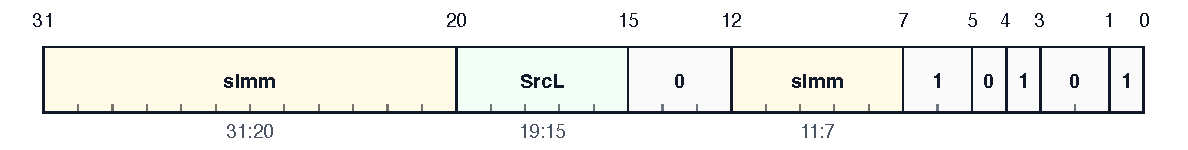
\includegraphics[width=\textwidth]{figs/encoding/scalar_instruction_entries/enc_sb_pcr.pdf}\par\smallskip
\begin{description}[leftmargin=0.18\linewidth,style=nextline]
\item[Format] \texttt{L32} \texttt{32-bit} scalar word.
\item[Pattern] \texttt{.................000.....1101001}.
\end{description}
\noindent\textbf{Classification.}\par
\begin{description}[leftmargin=0.18\linewidth,style=nextline]
\item[Category] Load, Store, and Address Generation.
\item[Family] Store Symbol.
\item[Execution class] \texttt{STA}; uop\_kind=AGU, agu\_kind=STA, split=AGU+STD.
\end{description}
\noindent\textbf{Operand fields.}\par
\begin{description}[leftmargin=0.18\linewidth,style=nextline]
\item[\texttt{SrcL}] Bits \texttt{19:15 (5b)}. 5-bit scalar source register used as the base address for the memory access.
\item[\texttt{simm}] Bits \texttt{31:20 (12b), 11:7 (5b)}. 17-bit signed address displacement added to the base register to form the effective address. The immediate is split across non-contiguous encoding slices and reassembled before use.
\end{description}
\noindent\textbf{Operation.}\par
\begin{lstlisting}[style=ptoscalarcode]
addr = ComputeAddress(/* per syntax */)
Store8(addr, Read(SrcL))
\end{lstlisting}
\Needspace{0.08\textheight}
